\documentclass[1p]{elsarticle_modified}
%\bibliographystyle{elsarticle-num}

%\usepackage[colorlinks]{hyperref}
%\usepackage{abbrmath_seonhwa} %\Abb, \Ascr, \Acal ,\Abf, \Afrak
\usepackage{amsfonts}
\usepackage{amssymb}
\usepackage{amsmath}
\usepackage{amsthm}
\usepackage{scalefnt}
\usepackage{amsbsy}
\usepackage{kotex}
\usepackage{caption}
\usepackage{subfig}
\usepackage{color}
\usepackage{graphicx}
\usepackage{xcolor} %% white, black, red, green, blue, cyan, magenta, yellow
\usepackage{float}
\usepackage{setspace}
\usepackage{hyperref}

\usepackage{tikz}
\usetikzlibrary{arrows}

\usepackage{multirow}
\usepackage{array} % fixed length table
\usepackage{hhline}

%%%%%%%%%%%%%%%%%%%%%
\makeatletter
\renewcommand*\env@matrix[1][\arraystretch]{%
	\edef\arraystretch{#1}%
	\hskip -\arraycolsep
	\let\@ifnextchar\new@ifnextchar
	\array{*\c@MaxMatrixCols c}}
\makeatother %https://tex.stackexchange.com/questions/14071/how-can-i-increase-the-line-spacing-in-a-matrix
%%%%%%%%%%%%%%%

\usepackage[normalem]{ulem}

\newcommand{\msout}[1]{\ifmmode\text{\sout{\ensuremath{#1}}}\else\sout{#1}\fi}
%SOURCE: \msout is \stkout macro in https://tex.stackexchange.com/questions/20609/strikeout-in-math-mode

\newcommand{\cancel}[1]{
	\ifmmode
	{\color{red}\msout{#1}}
	\else
	{\color{red}\sout{#1}}
	\fi
}

\newcommand{\add}[1]{
	{\color{blue}\uwave{#1}}
}

\newcommand{\replace}[2]{
	\ifmmode
	{\color{red}\msout{#1}}{\color{blue}\uwave{#2}}
	\else
	{\color{red}\sout{#1}}{\color{blue}\uwave{#2}}
	\fi
}

\newcommand{\Sol}{\mathcal{S}} %segment
\newcommand{\D}{D} %diagram
\newcommand{\A}{\mathcal{A}} %arc


%%%%%%%%%%%%%%%%%%%%%%%%%%%%%5 test

\def\sl{\operatorname{\textup{SL}}(2,\Cbb)}
\def\psl{\operatorname{\textup{PSL}}(2,\Cbb)}
\def\quan{\mkern 1mu \triangleright \mkern 1mu}

\theoremstyle{definition}
\newtheorem{thm}{Theorem}[section]
\newtheorem{prop}[thm]{Proposition}
\newtheorem{lem}[thm]{Lemma}
\newtheorem{ques}[thm]{Question}
\newtheorem{cor}[thm]{Corollary}
\newtheorem{defn}[thm]{Definition}
\newtheorem{exam}[thm]{Example}
\newtheorem{rmk}[thm]{Remark}
\newtheorem{alg}[thm]{Algorithm}

\newcommand{\I}{\sqrt{-1}}
\begin{document}

%\begin{frontmatter}
%
%\title{Boundary parabolic representations of knots up to 8 crossings}
%
%%% Group authors per affiliation:
%\author{Yunhi Cho} 
%\address{Department of Mathematics, University of Seoul, Seoul, Korea}
%\ead{yhcho@uos.ac.kr}
%
%
%\author{Seonhwa Kim} %\fnref{s_kim}}
%\address{Center for Geometry and Physics, Institute for Basic Science, Pohang, 37673, Korea}
%\ead{ryeona17@ibs.re.kr}
%
%\author{Hyuk Kim}
%\address{Department of Mathematical Sciences, Seoul National University, Seoul 08826, Korea}
%\ead{hyukkim@snu.ac.kr}
%
%\author{Seokbeom Yoon}
%\address{Department of Mathematical Sciences, Seoul National University, Seoul, 08826,  Korea}
%\ead{sbyoon15@snu.ac.kr}
%
%\begin{abstract}
%We find all boundary parabolic representation of knots up to 8 crossings.
%
%\end{abstract}
%\begin{keyword}
%    \MSC[2010] 57M25 
%\end{keyword}
%
%\end{frontmatter}

%\linenumbers
%\tableofcontents
%
\newcommand\colored[1]{\textcolor{white}{\rule[-0.35ex]{0.8em}{1.4ex}}\kern-0.8em\color{red} #1}%
%\newcommand\colored[1]{\textcolor{white}{ #1}\kern-2.17ex	\textcolor{white}{ #1}\kern-1.81ex	\textcolor{white}{ #1}\kern-2.15ex\color{red}#1	}

{\Large $\underline{10_{71}~(K10a_{10})}$}

\setlength{\tabcolsep}{10pt}
\renewcommand{\arraystretch}{1.6}
\vspace{1cm}\begin{tabular}{m{100pt}>{\centering\arraybackslash}m{274pt}}
\multirow{5}{120pt}{
	\centering
	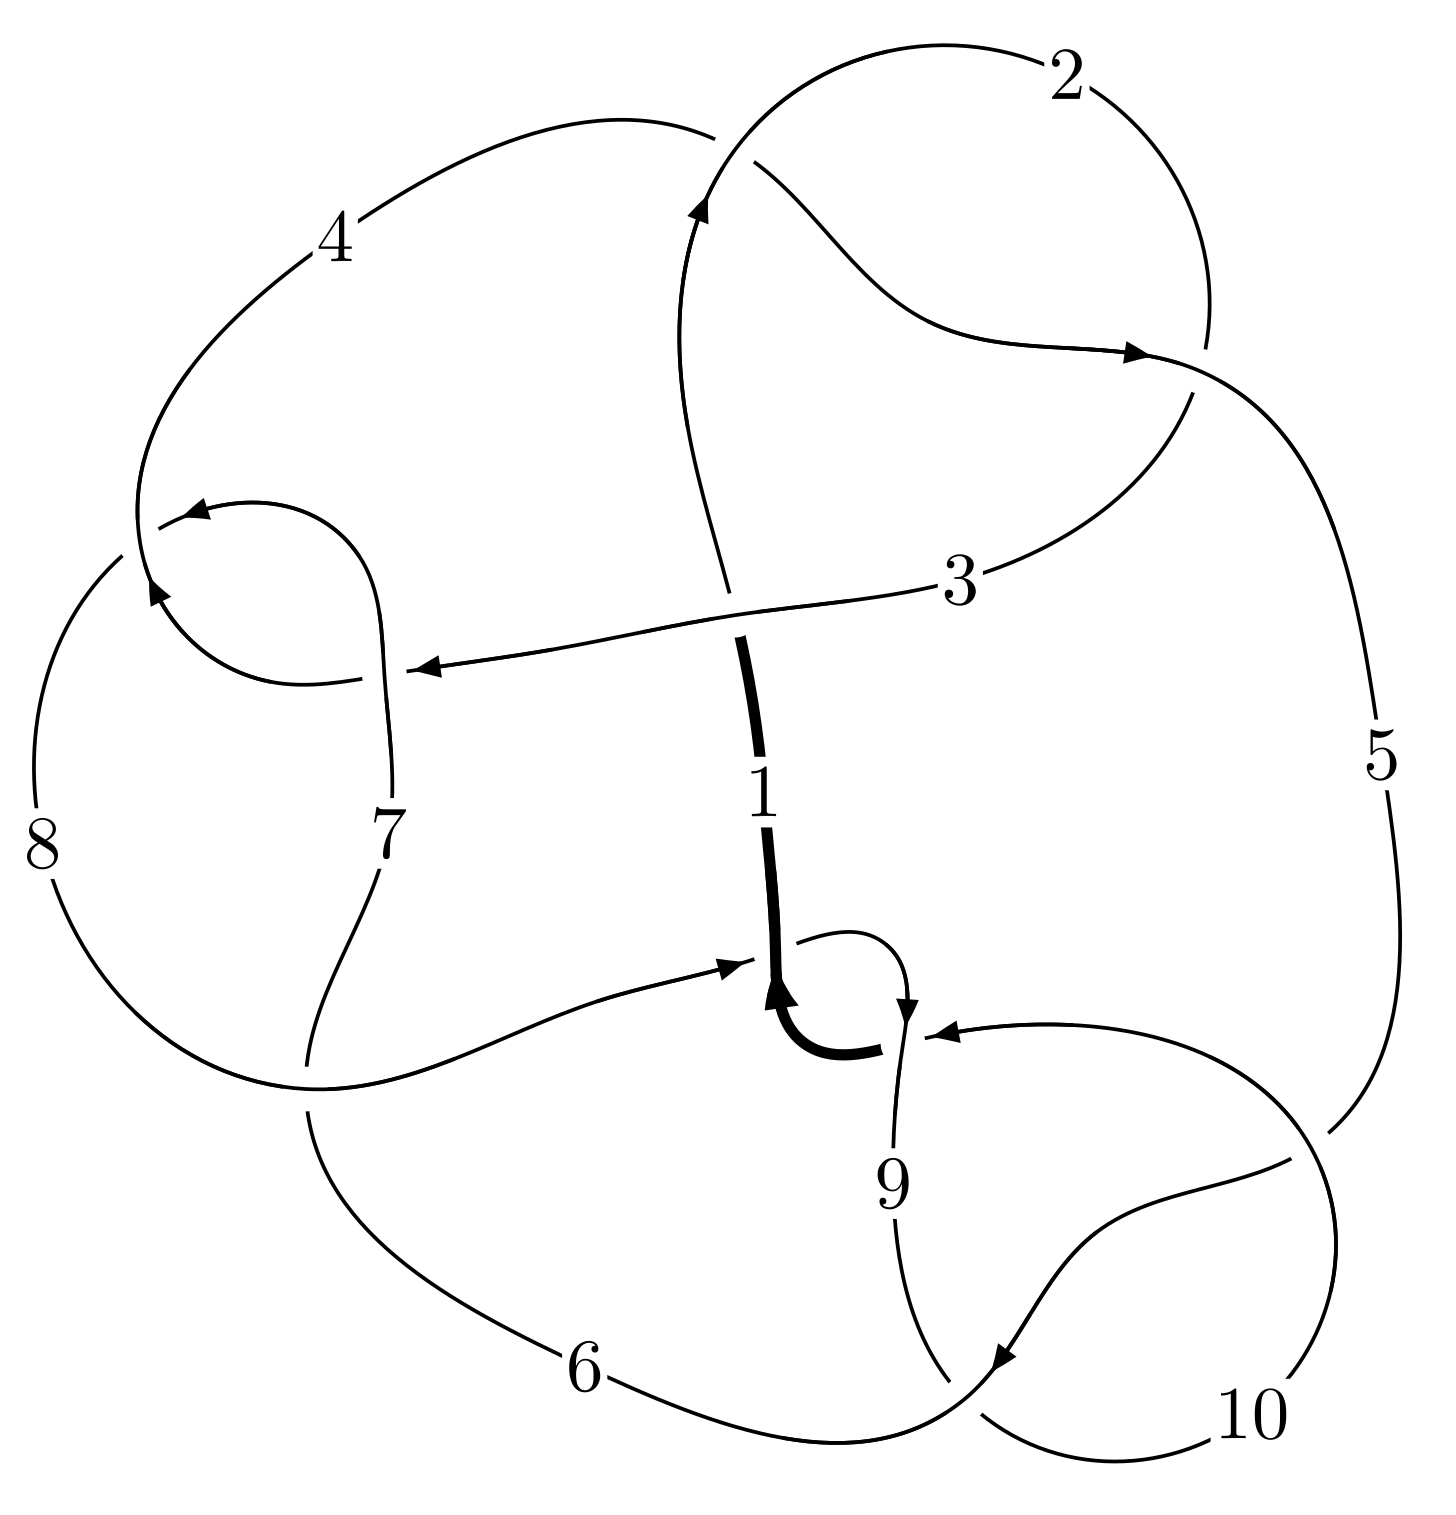
\includegraphics[width=112pt]{../../../GIT/diagram.site/Diagrams/png/155_10_71.png}\\
\ \ \ A knot diagram\footnotemark}&
\allowdisplaybreaks
\textbf{Linearized knot diagam} \\
\cline{2-2}
 &
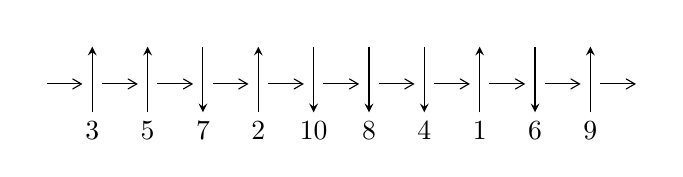
\begin{tikzpicture}[x=20pt, y=17pt]
	% nodes
	\node (C0) at (0, 0) {};
	\node (C1) at (1, 0) {};
	\node (C1U) at (1, +1) {};
	\node (C1D) at (1, -1) {3};

	\node (C2) at (2, 0) {};
	\node (C2U) at (2, +1) {};
	\node (C2D) at (2, -1) {5};

	\node (C3) at (3, 0) {};
	\node (C3U) at (3, +1) {};
	\node (C3D) at (3, -1) {7};

	\node (C4) at (4, 0) {};
	\node (C4U) at (4, +1) {};
	\node (C4D) at (4, -1) {2};

	\node (C5) at (5, 0) {};
	\node (C5U) at (5, +1) {};
	\node (C5D) at (5, -1) {10};

	\node (C6) at (6, 0) {};
	\node (C6U) at (6, +1) {};
	\node (C6D) at (6, -1) {8};

	\node (C7) at (7, 0) {};
	\node (C7U) at (7, +1) {};
	\node (C7D) at (7, -1) {4};

	\node (C8) at (8, 0) {};
	\node (C8U) at (8, +1) {};
	\node (C8D) at (8, -1) {1};

	\node (C9) at (9, 0) {};
	\node (C9U) at (9, +1) {};
	\node (C9D) at (9, -1) {6};

	\node (C10) at (10, 0) {};
	\node (C10U) at (10, +1) {};
	\node (C10D) at (10, -1) {9};
	\node (C11) at (11, 0) {};

	% arrows
	\draw[->,>={angle 60}]
	(C0) edge (C1) (C1) edge (C2) (C2) edge (C3) (C3) edge (C4) (C4) edge (C5) (C5) edge (C6) (C6) edge (C7) (C7) edge (C8) (C8) edge (C9) (C9) edge (C10) (C10) edge (C11) ;	\draw[->,>=stealth]
	(C1D) edge (C1U) (C2D) edge (C2U) (C3U) edge (C3D) (C4D) edge (C4U) (C5U) edge (C5D) (C6U) edge (C6D) (C7U) edge (C7D) (C8D) edge (C8U) (C9U) edge (C9D) (C10D) edge (C10U) ;
	\end{tikzpicture} \\
\hhline{~~} \\& 
\textbf{Solving Sequence} \\ \cline{2-2} 
 &
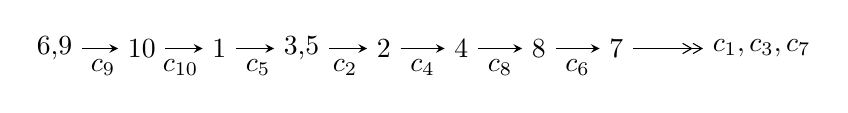
\begin{tikzpicture}[x=28pt, y=7pt]
	% node
	\node (A0) at (-1/8, 0) {6,9};
	\node (A1) at (1, 0) {10};
	\node (A2) at (2, 0) {1};
	\node (A3) at (49/16, 0) {3,5};
	\node (A4) at (33/8, 0) {2};
	\node (A5) at (41/8, 0) {4};
	\node (A6) at (49/8, 0) {8};
	\node (A7) at (57/8, 0) {7};
	\node (C1) at (1/2, -1) {$c_{9}$};
	\node (C2) at (3/2, -1) {$c_{10}$};
	\node (C3) at (5/2, -1) {$c_{5}$};
	\node (C4) at (29/8, -1) {$c_{2}$};
	\node (C5) at (37/8, -1) {$c_{4}$};
	\node (C6) at (45/8, -1) {$c_{8}$};
	\node (C7) at (53/8, -1) {$c_{6}$};
	\node (A8) at (9, 0) {$c_{1},c_{3},c_{7}$};

	% edge
	\draw[->,>=stealth]	
	(A0) edge (A1) (A1) edge (A2) (A2) edge (A3) (A3) edge (A4) (A4) edge (A5) (A5) edge (A6) (A6) edge (A7) ;
	\draw[->>,>={angle 60}]	
	(A7) edge (A8);
\end{tikzpicture} \\ 

\end{tabular} \\

\footnotetext{
The image of knot diagram is generated by the software ``\textbf{Draw programme}" developed by Andrew Bartholomew(\url{http://www.layer8.co.uk/maths/draw/index.htm\#Running-draw}), where we modified some parts for our purpose(\url{https://github.com/CATsTAILs/LinksPainter}).
}\phantom \\ \newline 
\centering \textbf{Ideals for irreducible components\footnotemark of $X_{\text{par}}$} 
 
\begin{align*}
I^u_{1}&=\langle 
u^{27}+5 u^{25}+\cdots+b+u,\;- u^{39}- u^{38}+\cdots+a-4 u,\;u^{40}+2 u^{39}+\cdots+4 u^2+1\rangle \\
I^u_{2}&=\langle 
b+u+1,\;a,\;u^2+u+1\rangle \\
\\
\end{align*}
\raggedright * 2 irreducible components of $\dim_{\mathbb{C}}=0$, with total 42 representations.\\
\footnotetext{All coefficients of polynomials are rational numbers. But the coefficients are sometimes approximated in decimal forms when there is not enough margin.}
\newpage
\renewcommand{\arraystretch}{1}
\centering \section*{I. $I^u_{1}= \langle u^{27}+5 u^{25}+\cdots+b+u,\;- u^{39}- u^{38}+\cdots+a-4 u,\;u^{40}+2 u^{39}+\cdots+4 u^2+1 \rangle$}
\flushleft \textbf{(i) Arc colorings}\\
\begin{tabular}{m{7pt} m{180pt} m{7pt} m{180pt} }
\flushright $a_{6}=$&$\begin{pmatrix}0\\u\end{pmatrix}$ \\
\flushright $a_{9}=$&$\begin{pmatrix}1\\0\end{pmatrix}$ \\
\flushright $a_{10}=$&$\begin{pmatrix}1\\u^2\end{pmatrix}$ \\
\flushright $a_{1}=$&$\begin{pmatrix}u^2+1\\u^2\end{pmatrix}$ \\
\flushright $a_{3}=$&$\begin{pmatrix}u^{39}+u^{38}+\cdots-5 u^2+4 u\\- u^{27}-5 u^{25}+\cdots+4 u^2- u\end{pmatrix}$ \\
\flushright $a_{5}=$&$\begin{pmatrix}u\\u^3+u\end{pmatrix}$ \\
\flushright $a_{2}=$&$\begin{pmatrix}u^{21}+4 u^{19}+\cdots-4 u^2+3 u\\- u^{39}-2 u^{38}+\cdots- u-1\end{pmatrix}$ \\
\flushright $a_{4}=$&$\begin{pmatrix}- u^{39}- u^{38}+\cdots+3 u-1\\-2 u^{39}-4 u^{38}+\cdots-4 u^2-2\end{pmatrix}$ \\
\flushright $a_{8}=$&$\begin{pmatrix}u^4+u^2+1\\u^4\end{pmatrix}$ \\
\flushright $a_{7}=$&$\begin{pmatrix}- u^9-2 u^7-3 u^5-2 u^3- u\\- u^9- u^7- u^5+u\end{pmatrix}$\\&\end{tabular}
\flushleft \textbf{(ii) Obstruction class $= -1$}\\~\\
\flushleft \textbf{(iii) Cusp Shapes $= u^{39}+9 u^{38}+17 u^{37}+66 u^{36}+94 u^{35}+285 u^{34}+329 u^{33}+852 u^{32}+826 u^{31}+1962 u^{30}+1576 u^{29}+3630 u^{28}+2362 u^{27}+5577 u^{26}+2755 u^{25}+7286 u^{24}+2421 u^{23}+8227 u^{22}+1323 u^{21}+8198 u^{20}-136 u^{19}+7289 u^{18}-1361 u^{17}+5878 u^{16}-1976 u^{15}+4322 u^{14}-1882 u^{13}+2864 u^{12}-1394 u^{11}+1700 u^{10}-826 u^9+838 u^8-385 u^7+329 u^6-157 u^5+92 u^4-42 u^3+7 u^2-5 u+6$}\\~\\
\newpage\renewcommand{\arraystretch}{1}
\flushleft \textbf{(iv) u-Polynomials at the component}\newline \\
\begin{tabular}{m{50pt}|m{274pt}}
Crossings & \hspace{64pt}u-Polynomials at each crossing \\
\hline $$\begin{aligned}c_{1}\end{aligned}$$&$\begin{aligned}
&u^{40}-21 u^{39}+\cdots-3 u+1
\end{aligned}$\\
\hline $$\begin{aligned}c_{2},c_{4}\end{aligned}$$&$\begin{aligned}
&u^{40}+3 u^{39}+\cdots+3 u+1
\end{aligned}$\\
\hline $$\begin{aligned}c_{3},c_{7}\end{aligned}$$&$\begin{aligned}
&u^{40}+u^{39}+\cdots-8 u+4
\end{aligned}$\\
\hline $$\begin{aligned}c_{5},c_{9}\end{aligned}$$&$\begin{aligned}
&u^{40}-2 u^{39}+\cdots+4 u^2+1
\end{aligned}$\\
\hline $$\begin{aligned}c_{6}\end{aligned}$$&$\begin{aligned}
&u^{40}+15 u^{39}+\cdots+120 u+16
\end{aligned}$\\
\hline $$\begin{aligned}c_{8},c_{10}\end{aligned}$$&$\begin{aligned}
&u^{40}-14 u^{39}+\cdots-8 u+1
\end{aligned}$\\
\hline
\end{tabular}\\~\\
\newpage\renewcommand{\arraystretch}{1}
\flushleft \textbf{(v) Riley Polynomials at the component}\newline \\
\begin{tabular}{m{50pt}|m{274pt}}
Crossings & \hspace{64pt}Riley Polynomials at each crossing \\
\hline $$\begin{aligned}c_{1}\end{aligned}$$&$\begin{aligned}
&y^{40}- y^{39}+\cdots+17 y+1
\end{aligned}$\\
\hline $$\begin{aligned}c_{2},c_{4}\end{aligned}$$&$\begin{aligned}
&y^{40}-21 y^{39}+\cdots-3 y+1
\end{aligned}$\\
\hline $$\begin{aligned}c_{3},c_{7}\end{aligned}$$&$\begin{aligned}
&y^{40}-15 y^{39}+\cdots-120 y+16
\end{aligned}$\\
\hline $$\begin{aligned}c_{5},c_{9}\end{aligned}$$&$\begin{aligned}
&y^{40}+14 y^{39}+\cdots+8 y+1
\end{aligned}$\\
\hline $$\begin{aligned}c_{6}\end{aligned}$$&$\begin{aligned}
&y^{40}+17 y^{39}+\cdots+2016 y+256
\end{aligned}$\\
\hline $$\begin{aligned}c_{8},c_{10}\end{aligned}$$&$\begin{aligned}
&y^{40}+26 y^{39}+\cdots+44 y+1
\end{aligned}$\\
\hline
\end{tabular}\\~\\
\newpage\flushleft \textbf{(vi) Complex Volumes and Cusp Shapes}
$$\begin{array}{c|c|c}  
\text{Solutions to }I^u_{1}& \I (\text{vol} + \sqrt{-1}CS) & \text{Cusp shape}\\
 \hline 
\begin{aligned}
u &= \phantom{-}0.725993 + 0.653238 I \\
a &= -1.77855 + 1.81598 I \\
b &= -2.56295 - 0.04821 I\end{aligned}
 & \phantom{-}0.63968 + 1.74616 I & \phantom{-}0.044303 - 1.257582 I \\ \hline\begin{aligned}
u &= \phantom{-}0.725993 - 0.653238 I \\
a &= -1.77855 - 1.81598 I \\
b &= -2.56295 + 0.04821 I\end{aligned}
 & \phantom{-}0.63968 - 1.74616 I & \phantom{-}0.044303 + 1.257582 I \\ \hline\begin{aligned}
u &= \phantom{-}0.657117 + 0.787048 I \\
a &= \phantom{-}1.66831 + 0.40061 I \\
b &= \phantom{-}0.89334 + 1.41707 I\end{aligned}
 & -1.07354 - 2.17702 I & -2.16670 + 4.43587 I \\ \hline\begin{aligned}
u &= \phantom{-}0.657117 - 0.787048 I \\
a &= \phantom{-}1.66831 - 0.40061 I \\
b &= \phantom{-}0.89334 - 1.41707 I\end{aligned}
 & -1.07354 + 2.17702 I & -2.16670 - 4.43587 I \\ \hline\begin{aligned}
u &= \phantom{-}0.096376 + 1.028080 I \\
a &= \phantom{-}0.442341 + 0.052565 I \\
b &= -0.722317 + 0.146557 I\end{aligned}
 & \phantom{-}2.32493 - 2.41163 I & \phantom{-}2.33571 + 3.34704 I \\ \hline\begin{aligned}
u &= \phantom{-}0.096376 - 1.028080 I \\
a &= \phantom{-}0.442341 - 0.052565 I \\
b &= -0.722317 - 0.146557 I\end{aligned}
 & \phantom{-}2.32493 + 2.41163 I & \phantom{-}2.33571 - 3.34704 I \\ \hline\begin{aligned}
u &= -0.824710 + 0.626683 I \\
a &= -1.67414 - 1.41541 I \\
b &= -2.39518 + 0.13829 I\end{aligned}
 & -1.20323 - 7.65538 I & -1.63964 + 4.86252 I \\ \hline\begin{aligned}
u &= -0.824710 - 0.626683 I \\
a &= -1.67414 + 1.41541 I \\
b &= -2.39518 - 0.13829 I\end{aligned}
 & -1.20323 + 7.65538 I & -1.63964 - 4.86252 I \\ \hline\begin{aligned}
u &= -0.789408 + 0.675423 I \\
a &= \phantom{-}1.235380 + 0.007261 I \\
b &= \phantom{-}1.156310 - 0.509552 I\end{aligned}
 & -3.72005 - 2.44717 I & -4.96365 + 1.04542 I \\ \hline\begin{aligned}
u &= -0.789408 - 0.675423 I \\
a &= \phantom{-}1.235380 - 0.007261 I \\
b &= \phantom{-}1.156310 + 0.509552 I\end{aligned}
 & -3.72005 + 2.44717 I & -4.96365 - 1.04542 I\\
 \hline 
 \end{array}$$\newpage$$\begin{array}{c|c|c}  
\text{Solutions to }I^u_{1}& \I (\text{vol} + \sqrt{-1}CS) & \text{Cusp shape}\\
 \hline 
\begin{aligned}
u &= \phantom{-}0.386153 + 0.965172 I \\
a &= -0.238506 + 0.455641 I \\
b &= -0.397991 + 0.639039 I\end{aligned}
 & \phantom{-}0.74845 - 2.81821 I & -1.95524 + 6.55211 I \\ \hline\begin{aligned}
u &= \phantom{-}0.386153 - 0.965172 I \\
a &= -0.238506 - 0.455641 I \\
b &= -0.397991 - 0.639039 I\end{aligned}
 & \phantom{-}0.74845 + 2.81821 I & -1.95524 - 6.55211 I \\ \hline\begin{aligned}
u &= -0.023616 + 1.041760 I \\
a &= -1.087150 - 0.838239 I \\
b &= \phantom{-}0.393277 - 1.005930 I\end{aligned}
 & \phantom{-}6.00686 + 1.32070 I & \phantom{-}7.28134 - 0.72610 I \\ \hline\begin{aligned}
u &= -0.023616 - 1.041760 I \\
a &= -1.087150 + 0.838239 I \\
b &= \phantom{-}0.393277 + 1.005930 I\end{aligned}
 & \phantom{-}6.00686 - 1.32070 I & \phantom{-}7.28134 + 0.72610 I \\ \hline\begin{aligned}
u &= -0.650732 + 0.672523 I \\
a &= \phantom{-}0.172779 + 0.250083 I \\
b &= -0.359504 - 0.987978 I\end{aligned}
 & \phantom{-}1.25887 + 0.68759 I & -0.543601 + 0.759704 I \\ \hline\begin{aligned}
u &= -0.650732 - 0.672523 I \\
a &= \phantom{-}0.172779 - 0.250083 I \\
b &= -0.359504 + 0.987978 I\end{aligned}
 & \phantom{-}1.25887 - 0.68759 I & -0.543601 - 0.759704 I \\ \hline\begin{aligned}
u &= \phantom{-}0.095598 + 1.116440 I \\
a &= -0.834103 + 0.849030 I \\
b &= \phantom{-}0.370183 + 0.684126 I\end{aligned}
 & \phantom{-}5.21580 - 6.90989 I & \phantom{-}5.24227 + 6.39245 I \\ \hline\begin{aligned}
u &= \phantom{-}0.095598 - 1.116440 I \\
a &= -0.834103 - 0.849030 I \\
b &= \phantom{-}0.370183 - 0.684126 I\end{aligned}
 & \phantom{-}5.21580 + 6.90989 I & \phantom{-}5.24227 - 6.39245 I \\ \hline\begin{aligned}
u &= \phantom{-}0.639866 + 0.934630 I \\
a &= -0.19632 + 1.43499 I \\
b &= -1.28155 + 0.60102 I\end{aligned}
 & -0.60920 - 2.86826 I & -1.22261 + 1.95241 I \\ \hline\begin{aligned}
u &= \phantom{-}0.639866 - 0.934630 I \\
a &= -0.19632 - 1.43499 I \\
b &= -1.28155 - 0.60102 I\end{aligned}
 & -0.60920 + 2.86826 I & -1.22261 - 1.95241 I\\
 \hline 
 \end{array}$$\newpage$$\begin{array}{c|c|c}  
\text{Solutions to }I^u_{1}& \I (\text{vol} + \sqrt{-1}CS) & \text{Cusp shape}\\
 \hline 
\begin{aligned}
u &= -0.777168 + 0.837928 I \\
a &= -0.91272 - 1.60741 I \\
b &= -2.00597 - 0.19942 I\end{aligned}
 & -6.21108 + 0.22925 I & -5.84725 + 0.24543 I \\ \hline\begin{aligned}
u &= -0.777168 - 0.837928 I \\
a &= -0.91272 + 1.60741 I \\
b &= -2.00597 + 0.19942 I\end{aligned}
 & -6.21108 - 0.22925 I & -5.84725 - 0.24543 I \\ \hline\begin{aligned}
u &= -0.762796 + 0.899428 I \\
a &= \phantom{-}1.74060 + 0.53261 I \\
b &= \phantom{-}2.07413 - 1.05941 I\end{aligned}
 & -6.02457 + 5.56367 I & -5.18066 - 6.01609 I \\ \hline\begin{aligned}
u &= -0.762796 - 0.899428 I \\
a &= \phantom{-}1.74060 - 0.53261 I \\
b &= \phantom{-}2.07413 + 1.05941 I\end{aligned}
 & -6.02457 - 5.56367 I & -5.18066 + 6.01609 I \\ \hline\begin{aligned}
u &= -0.651476 + 0.987984 I \\
a &= \phantom{-}0.197553 + 0.008658 I \\
b &= -0.673463 - 1.012420 I\end{aligned}
 & \phantom{-}2.21178 + 4.43619 I & \phantom{-}1.72906 - 5.48285 I \\ \hline\begin{aligned}
u &= -0.651476 - 0.987984 I \\
a &= \phantom{-}0.197553 - 0.008658 I \\
b &= -0.673463 + 1.012420 I\end{aligned}
 & \phantom{-}2.21178 - 4.43619 I & \phantom{-}1.72906 + 5.48285 I \\ \hline\begin{aligned}
u &= \phantom{-}0.559538 + 1.043730 I \\
a &= \phantom{-}0.204110 + 0.051194 I \\
b &= -0.743272 + 0.884629 I\end{aligned}
 & \phantom{-}2.37466 + 0.03317 I & \phantom{-}2.30074 - 1.92960 I \\ \hline\begin{aligned}
u &= \phantom{-}0.559538 - 1.043730 I \\
a &= \phantom{-}0.204110 - 0.051194 I \\
b &= -0.743272 - 0.884629 I\end{aligned}
 & \phantom{-}2.37466 - 0.03317 I & \phantom{-}2.30074 + 1.92960 I \\ \hline\begin{aligned}
u &= \phantom{-}0.674430 + 1.003370 I \\
a &= \phantom{-}1.99901 - 1.47152 I \\
b &= \phantom{-}3.05304 + 1.06309 I\end{aligned}
 & \phantom{-}1.68055 - 7.12390 I & \phantom{-}1.84913 + 6.13601 I \\ \hline\begin{aligned}
u &= \phantom{-}0.674430 - 1.003370 I \\
a &= \phantom{-}1.99901 + 1.47152 I \\
b &= \phantom{-}3.05304 - 1.06309 I\end{aligned}
 & \phantom{-}1.68055 + 7.12390 I & \phantom{-}1.84913 - 6.13601 I\\
 \hline 
 \end{array}$$\newpage$$\begin{array}{c|c|c}  
\text{Solutions to }I^u_{1}& \I (\text{vol} + \sqrt{-1}CS) & \text{Cusp shape}\\
 \hline 
\begin{aligned}
u &= \phantom{-}0.710235 + 0.337827 I \\
a &= \phantom{-}0.496293 - 0.392962 I \\
b &= -0.069099 + 0.837495 I\end{aligned}
 & \phantom{-}0.39800 - 4.72692 I & -1.63267 + 6.05913 I \\ \hline\begin{aligned}
u &= \phantom{-}0.710235 - 0.337827 I \\
a &= \phantom{-}0.496293 + 0.392962 I \\
b &= -0.069099 - 0.837495 I\end{aligned}
 & \phantom{-}0.39800 + 4.72692 I & -1.63267 - 6.05913 I \\ \hline\begin{aligned}
u &= -0.705098 + 1.010600 I \\
a &= -0.462757 - 1.241560 I \\
b &= -1.290960 - 0.160212 I\end{aligned}
 & -2.70648 + 8.09252 I & -2.94350 - 6.08172 I \\ \hline\begin{aligned}
u &= -0.705098 - 1.010600 I \\
a &= -0.462757 + 1.241560 I \\
b &= -1.290960 + 0.160212 I\end{aligned}
 & -2.70648 - 8.09252 I & -2.94350 + 6.08172 I \\ \hline\begin{aligned}
u &= -0.703890 + 1.042830 I \\
a &= \phantom{-}1.61753 + 1.43395 I \\
b &= \phantom{-}2.91214 - 0.75501 I\end{aligned}
 & \phantom{-}0.05370 + 13.38520 I & \phantom{-}0.42075 - 9.35928 I \\ \hline\begin{aligned}
u &= -0.703890 - 1.042830 I \\
a &= \phantom{-}1.61753 - 1.43395 I \\
b &= \phantom{-}2.91214 + 0.75501 I\end{aligned}
 & \phantom{-}0.05370 - 13.38520 I & \phantom{-}0.42075 + 9.35928 I \\ \hline\begin{aligned}
u &= \phantom{-}0.566007 + 0.177460 I \\
a &= \phantom{-}0.944370 + 0.216688 I \\
b &= \phantom{-}0.239645 - 0.184623 I\end{aligned}
 & -1.47568 - 0.52119 I & -6.28438 + 0.91978 I \\ \hline\begin{aligned}
u &= \phantom{-}0.566007 - 0.177460 I \\
a &= \phantom{-}0.944370 - 0.216688 I \\
b &= \phantom{-}0.239645 + 0.184623 I\end{aligned}
 & -1.47568 + 0.52119 I & -6.28438 - 0.91978 I \\ \hline\begin{aligned}
u &= -0.222419 + 0.359701 I \\
a &= -0.03404 + 1.68269 I \\
b &= -0.589808 - 0.653481 I\end{aligned}
 & \phantom{-}1.75548 + 0.68997 I & \phantom{-}4.17661 + 0.16492 I \\ \hline\begin{aligned}
u &= -0.222419 - 0.359701 I \\
a &= -0.03404 - 1.68269 I \\
b &= -0.589808 + 0.653481 I\end{aligned}
 & \phantom{-}1.75548 - 0.68997 I & \phantom{-}4.17661 - 0.16492 I\\
 \hline 
 \end{array}$$\newpage\newpage\renewcommand{\arraystretch}{1}
\centering \section*{II. $I^u_{2}= \langle b+u+1,\;a,\;u^2+u+1 \rangle$}
\flushleft \textbf{(i) Arc colorings}\\
\begin{tabular}{m{7pt} m{180pt} m{7pt} m{180pt} }
\flushright $a_{6}=$&$\begin{pmatrix}0\\u\end{pmatrix}$ \\
\flushright $a_{9}=$&$\begin{pmatrix}1\\0\end{pmatrix}$ \\
\flushright $a_{10}=$&$\begin{pmatrix}1\\- u-1\end{pmatrix}$ \\
\flushright $a_{1}=$&$\begin{pmatrix}- u\\- u-1\end{pmatrix}$ \\
\flushright $a_{3}=$&$\begin{pmatrix}0\\- u-1\end{pmatrix}$ \\
\flushright $a_{5}=$&$\begin{pmatrix}u\\u+1\end{pmatrix}$ \\
\flushright $a_{2}=$&$\begin{pmatrix}- u\\-2 u-2\end{pmatrix}$ \\
\flushright $a_{4}=$&$\begin{pmatrix}0\\- u-1\end{pmatrix}$ \\
\flushright $a_{8}=$&$\begin{pmatrix}0\\u\end{pmatrix}$ \\
\flushright $a_{7}=$&$\begin{pmatrix}0\\u\end{pmatrix}$\\&\end{tabular}
\flushleft \textbf{(ii) Obstruction class $= 1$}\\~\\
\flushleft \textbf{(iii) Cusp Shapes $= -4 u+1$}\\~\\
\newpage\renewcommand{\arraystretch}{1}
\flushleft \textbf{(iv) u-Polynomials at the component}\newline \\
\begin{tabular}{m{50pt}|m{274pt}}
Crossings & \hspace{64pt}u-Polynomials at each crossing \\
\hline $$\begin{aligned}c_{1},c_{2}\end{aligned}$$&$\begin{aligned}
&(u+1)^2
\end{aligned}$\\
\hline $$\begin{aligned}c_{3},c_{6},c_{7}\end{aligned}$$&$\begin{aligned}
&u^2
\end{aligned}$\\
\hline $$\begin{aligned}c_{4}\end{aligned}$$&$\begin{aligned}
&(u-1)^2
\end{aligned}$\\
\hline $$\begin{aligned}c_{5},c_{10}\end{aligned}$$&$\begin{aligned}
&u^2- u+1
\end{aligned}$\\
\hline $$\begin{aligned}c_{8},c_{9}\end{aligned}$$&$\begin{aligned}
&u^2+u+1
\end{aligned}$\\
\hline
\end{tabular}\\~\\
\newpage\renewcommand{\arraystretch}{1}
\flushleft \textbf{(v) Riley Polynomials at the component}\newline \\
\begin{tabular}{m{50pt}|m{274pt}}
Crossings & \hspace{64pt}Riley Polynomials at each crossing \\
\hline $$\begin{aligned}c_{1},c_{2},c_{4}\end{aligned}$$&$\begin{aligned}
&(y-1)^2
\end{aligned}$\\
\hline $$\begin{aligned}c_{3},c_{6},c_{7}\end{aligned}$$&$\begin{aligned}
&y^2
\end{aligned}$\\
\hline $$\begin{aligned}c_{5},c_{8},c_{9}\\c_{10}\end{aligned}$$&$\begin{aligned}
&y^2+y+1
\end{aligned}$\\
\hline
\end{tabular}\\~\\
\newpage\flushleft \textbf{(vi) Complex Volumes and Cusp Shapes}
$$\begin{array}{c|c|c}  
\text{Solutions to }I^u_{2}& \I (\text{vol} + \sqrt{-1}CS) & \text{Cusp shape}\\
 \hline 
\begin{aligned}
u &= -0.500000 + 0.866025 I \\
a &= \phantom{-0.000000 } 0 \\
b &= -0.500000 - 0.866025 I\end{aligned}
 & \phantom{-}1.64493 + 2.02988 I & \phantom{-}3.00000 - 3.46410 I \\ \hline\begin{aligned}
u &= -0.500000 - 0.866025 I \\
a &= \phantom{-0.000000 } 0 \\
b &= -0.500000 + 0.866025 I\end{aligned}
 & \phantom{-}1.64493 - 2.02988 I & \phantom{-}3.00000 + 3.46410 I\\
 \hline 
 \end{array}$$\newpage
\newpage\renewcommand{\arraystretch}{1}
\centering \section*{ III. u-Polynomials}
\begin{tabular}{m{50pt}|m{274pt}}
Crossings & \hspace{64pt}u-Polynomials at each crossing \\
\hline $$\begin{aligned}c_{1}\end{aligned}$$&$\begin{aligned}
&((u+1)^2)(u^{40}-21 u^{39}+\cdots-3 u+1)
\end{aligned}$\\
\hline $$\begin{aligned}c_{2}\end{aligned}$$&$\begin{aligned}
&((u+1)^2)(u^{40}+3 u^{39}+\cdots+3 u+1)
\end{aligned}$\\
\hline $$\begin{aligned}c_{3},c_{7}\end{aligned}$$&$\begin{aligned}
&u^2(u^{40}+u^{39}+\cdots-8 u+4)
\end{aligned}$\\
\hline $$\begin{aligned}c_{4}\end{aligned}$$&$\begin{aligned}
&((u-1)^2)(u^{40}+3 u^{39}+\cdots+3 u+1)
\end{aligned}$\\
\hline $$\begin{aligned}c_{5}\end{aligned}$$&$\begin{aligned}
&(u^2- u+1)(u^{40}-2 u^{39}+\cdots+4 u^2+1)
\end{aligned}$\\
\hline $$\begin{aligned}c_{6}\end{aligned}$$&$\begin{aligned}
&u^2(u^{40}+15 u^{39}+\cdots+120 u+16)
\end{aligned}$\\
\hline $$\begin{aligned}c_{8}\end{aligned}$$&$\begin{aligned}
&(u^2+u+1)(u^{40}-14 u^{39}+\cdots-8 u+1)
\end{aligned}$\\
\hline $$\begin{aligned}c_{9}\end{aligned}$$&$\begin{aligned}
&(u^2+u+1)(u^{40}-2 u^{39}+\cdots+4 u^2+1)
\end{aligned}$\\
\hline $$\begin{aligned}c_{10}\end{aligned}$$&$\begin{aligned}
&(u^2- u+1)(u^{40}-14 u^{39}+\cdots-8 u+1)
\end{aligned}$\\
\hline
\end{tabular}\newpage\renewcommand{\arraystretch}{1}
\centering \section*{ IV. Riley Polynomials}
\begin{tabular}{m{50pt}|m{274pt}}
Crossings & \hspace{64pt}Riley Polynomials at each crossing \\
\hline $$\begin{aligned}c_{1}\end{aligned}$$&$\begin{aligned}
&((y-1)^2)(y^{40}- y^{39}+\cdots+17 y+1)
\end{aligned}$\\
\hline $$\begin{aligned}c_{2},c_{4}\end{aligned}$$&$\begin{aligned}
&((y-1)^2)(y^{40}-21 y^{39}+\cdots-3 y+1)
\end{aligned}$\\
\hline $$\begin{aligned}c_{3},c_{7}\end{aligned}$$&$\begin{aligned}
&y^2(y^{40}-15 y^{39}+\cdots-120 y+16)
\end{aligned}$\\
\hline $$\begin{aligned}c_{5},c_{9}\end{aligned}$$&$\begin{aligned}
&(y^2+y+1)(y^{40}+14 y^{39}+\cdots+8 y+1)
\end{aligned}$\\
\hline $$\begin{aligned}c_{6}\end{aligned}$$&$\begin{aligned}
&y^2(y^{40}+17 y^{39}+\cdots+2016 y+256)
\end{aligned}$\\
\hline $$\begin{aligned}c_{8},c_{10}\end{aligned}$$&$\begin{aligned}
&(y^2+y+1)(y^{40}+26 y^{39}+\cdots+44 y+1)
\end{aligned}$\\
\hline
\end{tabular}
\vskip 2pc
\end{document}